%\setcounter{section}{0}
%\setcounter{subsection}{0}
%\setcounter{subsubsection}{0}
%\setcounter{equation}{0}
%\setcounter{page}{0} 
%\pagenumbering{arabic} 
%\setcounter{page}{1}    %%%%%KKD used \setcounter{page}{0}  
%\oddsidemargin 0.9 cm 
%\evensidemargin -.4 cm
%\setlength{\textwidth}{152.4 mm}
\setcounter{section}{3}
\setcounter{subsection}{3}
\setcounter{subsubsection}{3}
\setcounter{equation}{3}
\chapter{Beyond the Standard Model  \label{Beyond the Standard Model}}
Physics beyond the standard model (BSM)~\cite{bsm} refers to the theoretical proposals put forward to explain deficiencies of the SM. BSM models include various supersymmetric extensions ~\cite{SUSYprimer}, such as the Minimal Supersymmetric Standard Model (MSSM)~\cite{MSSMref} and Next-to-Minimal Supersymmetric Standard Model (NMSSM)~\cite{NMSSMref}, Leptoquark models or entirely novel explanations deriving from string theory such as extra dimensions~\cite{extra-dim}. In the following sections we will discuss about supersymmetry (SUSY) and Leptoquark models. 

\section{Supersymmetry}
Supersymmetry (SUSY) is one of the proposed extensions to the SM that introduces a new kind of space-time symmetry and relates two classes of elementary particles: bosons and fermions. In this model, each SM particle has its so called superpartner differing by spin $\frac{1}{2}$. If supersymmetry were unbroken, all the SUSY partners would have the same mass as the corresponding SM particles. The fact that no SUSY particles have been found, tells us that it must be a broken symmetry. SUSY solves many outstanding problems in particle physics including the hierarchy problem. The simplest realization of the broken SUSY is MSSM. As described earlier, a supersymmetric transformation converts a bosonic state to a fermionic state and vice versa. If ${\rm \bf Q}$ denotes such an operator then 
%\begin{equation}\label{SUSYtransform}

 $\rm {\bf Q}| Boson>  =  | Fermion>, {\bf Q}| Fermion> =  | Boson> $
%\end{equation}

%, $Q|\rm Fermion> =  | Boson>$
%$\rm Q| Boson>$  = $ | Fermion>$
with {\bf Q} being an anti-commuting spinor. The supersymmetric partner of fermion is called a sfermion. For instance, quarks have squarks and leptons have  sleptons. The left- and right-handed components of the quarks and leptons are distinct two-component Weyl fermions with different gauge transformation properties in the SM, so each must have its own complex scalar partner. The symbols for  squarks and sleptons are the same as for the corresponding fermion, but with a tilde $\sim$ used to denote the superpartner of a SM particle. As an example, the superpartners of the left- and right-handed components of the electron Dirac field are called left- and right-handed selectrons, and are denoted $\tilde{e}_{L}$ and $\tilde{e}_{R}$ respectively. Here, the handedness does not refer to the helicity of selectrons. As the neutrinos are always left-handed they are denoted just by $\tilde{\nu_{e}}$,$\tilde{\nu_{\tau}}$ and $\tilde{\nu_{\mu}}$. Similarly, for the quarks they are given by $\tilde{q}_{L}$ and $\tilde{q}_{R}$, where $q$ stands for six types of quarks. Theories show that the Higgs cannot reside in a single supermultiplet. So there are two Higgs supermupliplets with Y=$\pm \frac{1}{2}$. We will call the $\rm SU(2)_{L}$-doublet complex scalar fields with  Y=$+ \frac{1}{2}$ and Y=$- \frac{1}{2}$ by the names $H_{u}$ and $H_{d}$, respectively. The superpartners of Higgs are called higgsinos. The weak isospin components of $H_{u}$ with $T_{3}$ = ($\frac{1}{2}$, -$\frac{1}{2}$) have electric charges 1 and 0, respectively, and are denoted by ($H_{u}^{+}$, $H_{u}^{0}$). The neutral scalar that corresponds to the physical
SM Higgs boson is in a linear combination of $H_{u}^{0}$ and $H_{d}^{0}$. Higgsinos are denoted as $\tilde{H}_{u}$, $\tilde{H}_{d}$ for the $\rm SU(2)_{L}$ doublet left-handed Weyl spinor fields, with weak isospin components ($\tilde{H}_{u}^{+}$ and $\tilde{H}_{u}^{0}$) and ($\tilde{H}_{d}^{0}$ and $\tilde{H}_{d}^{-}$). Similarly the superpartner of gluon($g$) is gluino ($\tilde{g}$). The electroweak gauge symmetry $SU(2)_{L} \otimes U(1)_{Y}$ is associated with spin-1 gauge bosons $W^{\pm}$, $W^{0}$ and $B^{0}$ with spin $\frac{1}{2}$ superpartners $\tilde{W}^{\pm}$, $\tilde{W}^{0}$ and $\tilde{B}^{0}$, called winos and bino. After electroweak symmetry breaking the  $W^{0}$ and $B^{0}$ eigenstates mix to give mass eigen states $Z^{0}$ and $\gamma$. The corresponding gaugino mixtures of $\tilde{W}^{0}$ and $\tilde{B}^{0}$ are called zino ($\tilde{Z}^{0}$) and photino ($\tilde{\gamma}$). A list of SUSY and SM particles  in the context of MSSM is given in Table.~\ref{tab:mssmspec}. They are also pictorially shown 
in Fig.~\ref{fig:SMandSUSYparticles}.


\begin{table}[h]
\begin{center}
\caption{Field content of MSSM in terms of superfields(1st column), sparticles and SM particles(2nd and 3rd column) while  in the  4th column the quantum numbers for various fields are shown.}
 \begin{tabular}{||c c c c||}
 \hline
 Supermultiplet & S=0 or 1& S=1/2 & $SU(3),SU(2)_L,U(1)_Y$ \\ [0.5ex]
 \hline\hline
                 &squarks                   & quarks     &  \\
    Q            &$(\tilde u_L,\tilde d_L)$  & $(u_L, d_L)$  &($3,2,1/6$)  \\
   $\bar U$      & $\tilde u^*_R$ &$ u^{\dagger}_R$  & ($\bar 3, 1,-2/3$) \\
  $\bar D $      & $\tilde d^*_R$ & $d^{\dagger}_R$  & ($\bar 3, 1, 1/3$) \\  \hline
                 &sleptons                   & leptons   &  \\
    L            & $(\tilde \nu_L, \tilde e_L)$ &$(\nu_L, e_L) $ & ($1,2,-1/2$) \\
   $\bar E$      & $\tilde e^*_R$ & $e^{\dagger}_R$  & $(1,1,1)$ \\ \hline
                 &Higgs                         &Higgsino &    \\
    $H_u$        & ($H_u^+,H_u^0$) &($\tilde H_u^+,\tilde H_u^0$)  & ($1,2,1/2$) \\
    $H_d$        & ($H_d^0,H_d^-$) &($\tilde H_d^0,\tilde H_d^-$)  & ($1,2,-1/2$) \\   \hline
                 & gauge bosons    & gaugino   &  \\
    $V^(y)$        & $B_{\mu}$   &$\tilde B_{\mu}$  & ($1,1,-$) \\
    $V^{a(2)}$     & $W_{\mu}^a$ &$\tilde W_{\mu}^a$ & ($3,1,-$) \\   \hline
    $V^{a(3)}$     & $g_{\mu}^a$ &$\tilde g_{\mu}^a$  & ($8,1,-$) \\   \hline
\end{tabular}

\label{tab:mssmspec}
\end{center}
\end{table}



\begin{figure}[h]
    \centering
    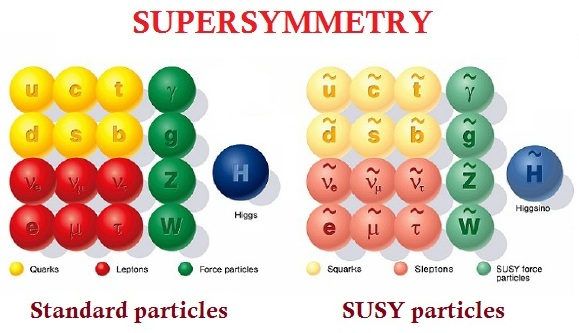
\includegraphics[width=15.0cm,height=8cm]{/home/bibhu/Desktop/PhDThesis/PhDThesis/chapter3/SMandSUSYparticles.jpg}
    \caption{ \small SM and their SUSY partners.}
    \label{fig:SMandSUSYparticles}
\end{figure}

In the framework of MSSM with R-parity~\cite{RParity} conservation, SUSY particles are produced in pairs. At LHC, the most abundantly produced SUSY particles are expected to be strongly interacting partners of quarks and gluons, i.e. the squarks and gluinos. The dominant gluino and squark production processes are 	


$pp\rightarrow \tilde{g}\tilde{g}+X, \tilde{q}\tilde{g}, \tilde{q}\tilde{q}, \tilde{q}\tilde{q}^{*}$

In our SUSY analysis, we mainly focus on gluino pair production because it has largest cross section for squark decoupling simplified scenarios~\cite{XsecSUSY}. Simplified SUSY models, also called ``simplified model space'' (SMS), try to reduce the complex parameter space of SUSY to a minimal number so that it would be easier for the experimentalists to interpret data and derive limits on the cross sections. The SMS models used in our analysis have two free parameters, namely the gluino and lightest SUSY particle (LSP) mass. Other particles are considered to be too heavy to participate in the process.~\cite{xsecGlu,XsecSUSY,SMS1} 


\newpage
\section{Leptoquark models}

Leptoquarks are scalar or vector particles that carry information back and forth between quarks and leptons of a given generation allowing them  to interact. They are color-triplet bosons and carry both lepton and baryon numbers. They appear in various extensions of the SM, such as technicolor ~\cite{technicolor2, technicolor3,LQ2} or grand unified theories based on Pati-Salam model~\cite{LQ3}, SU(5)~\cite{LQ4} or E6~\cite{superstring_e6} or composite models~\cite{composite}. Leptoquarks explain why there are three generations of matter. Therefore, they provide very useful information to either falsify or exclude the parameter space of BSM theories. In the search we will be describing later, we look for first generation scalar leptoquarks. We list different scalar leptoquark models in Table~\ref{tab:scalarLeptoQuark}. We follow the notation from Ref.~\cite{pdg1}.



\begin{table}[h]
\begin{center}
\caption{Quantum numbers of scalar leptoquarks and possible renormalizable interactions
containing them. We take the table from Ref.~\cite{LQLHC}.}
 \begin{tabular}{||c c c||}
 \hline
 Leptoquark & Renormalizable couplings & $SU(3)_{C} \otimes SU(2)_L \otimes U(1)_Y$ \\ [0.5ex]
 \hline\hline
                 &       &  \\
                  $S_{0}$     &$S_{0}Q_{L}^{\dagger}, S_{0}u_{R}^{\dagger}e_{R}^{\dagger}, S_{0}Q_{L}Q_{L}$   &  (${\bf 3},{\bf 1},-1/3$)  \\
           $\tilde{S_{0}} $   & $\tilde{S_{0}}d_{R}^{\dagger}e_{R}^{\dagger}, \tilde{S_{0}}u_{R}u_{R}$             &  (${\bf 3},{\bf 1},-4/3$) \\
                   $S_{1} $   & $S_{1}Q_{L}^{\dagger},L_{L}^{\dagger}, S_{1}Q_{L}Q_{L}$             &  (${\bf 3},{\bf  3}, -1/3$) \\  
        $S^{\dagger}_{1/2} $  & $S_{1/2}^{\dagger}Q_{L}^{\dagger}e_{R}, S_{1/2}^{\dagger}u_{R}^{\dagger}L_{L} $             &  (${\bf 3},{\bf  2}, +7/6$) \\  
  $\tilde{S}^{\dagger}_{1/2}$ & $\tilde{S}_{1/2}^{\dagger}d_{R}^{\dagger}L_{L}$             &  (${\bf 3},{\bf  2}, +1/6$) \\  \hline
  

\end{tabular}
\label{tab:scalarLeptoQuark}
\end{center}
\end{table}












